\chapter{Resultados}
    \section{Implementación}
    Para lograr los objetivos planteados para el desarrollo de este proyecto se utilizaron varias herramientas de software y de hardware, las cuales hicieron posible la recopilación de los datos necesarios, así como la ejecución de las acciones planteadas como requisitos del proceso planteado.
    Se ha hecho suficiente hincapié en que el objetivo principal de este proyecto es el aprovechamiento de los datos recabados por una cámara RGBD. En este caso, el dispositivo utilizado para la obtención de la imagen y la nube de puntos es el \textbf{Kinect}, un dispositivo distribuido por la empresa \textbf{Microsoft}, que en 2010 fue lanzado al mercado como accesorio para la consola de videojuegos XBOX 360. Adicionalmente, como base del robot móvil se utilizó la plataforma de desarrollo \textbf{Robotino} perteneciente a la empresa FESTO.

    
        \subsection{Herramientas de software}
            \subsubsection{ROS}
            En 2018 Edgar Vázquez realiza una breve de descripción del sistema ROS, en la cual comenta que el objetivo principal es dar soporte a la reutilización de código en la investigación y desarrollo de robótica, referenciando a Quigley en \cite{quigley_ROS}. Adicionalmente, Vázquez menciona que ROS ofrece las siguientes utilidades:
            \begin{itemize}
                \item Abstracción de hardware
                \item Control de dispositivos de bajo nivel
                \item Implementación de funcionalidades comunes entre dispositivos
                \item Intercambio de mensajes entre procesos
                \item Mantenimiento de paquetes
            \end{itemize}

            Vázquez añade que durante el desarrollo del comportamiento de un robot es común considerar las funcionalidades a modo de módulos, en que cada uno tiene un objetivo específico. Apunta también que ROS colabora con el transporte de la información entre dichos módulos y menciona como una ventaja la existencia de la comunidad de desarrolladores que trabajan con ROS, haciendo posible el intercambio de información, obteniendo soporte y retroalimentación actualizados.
            \phantom{saltodelineaforzado >:D}\\

            \textbf{Elementos}
            \begin{itemize}
                \item Nodos: los nodos son los módulos que en conjunto forman la red le trabajo, y se encargar generalmente de las funcionalidades aisladas que se mencionaron anteriormente. Es decir, la activación de los actuadores, el procesamiento de imagen, el control de la interfaz del usuario, cada una de estas actividades se encontraría bajo el cargo de un nodo, independiente de las demás, pero que bajo la estructura de ROS les es posible intercambiar información.
                \item Paquetes: Vázquez comenta que dentro de la estructura de ROS, los paquetes pueden se comparados con carpetas, las cuales tienen características estructurales definidas y en las cuales es posible contener a los nodos. Además, dentro del paquete se deben establecer las bibliotecas u otras paqueterías que requiera la correcta ejecución de los nodos, como pueden ser los tipos de datos personalizados, recursos ajenos a ROS o archivos de configuración adicionales. 
                \item Tópicos: son el elemento que se utiliza para intercomunicar los nodos. Dentro de la implementación con ROS es posible \textit{publicar} información dentro del entorno por medio de mensajes y haciendo uso de los tópicos, los mensajes pueden ser diversos tipos, dependiendo de los requerimientos de la implementación, adicionalmente, es posible crear nuevos tipos de mensaje de ser necesario \cite{ros_wiki_std_msgs}. 
                \item Servicios: un método distinto a los tópicos mediante el cual también se puede compartir información son los servicios. La diferencia entre estas herramientas es que los servicios necesitan ser solicitados por otro agente, es decir, sigue un modelo petición-respuesta. Vázquez comenta que si un proceso necesita realizarse solo en momentos específicos lo recomendable es implementarlo como un servicio.
            \end{itemize}

            
            \subsubsection{OpenCV}
            \textit{The Open Source Computer Vision Library}, se trata de una biblioteca de acceso libre a través de la cual es posible utilizar cientos de algoritmos de procesamiento de imágenes y visión computacional.
            
            Dentro de la información que ofrece el sitio web de la biblioteca, se menciona que cuenta con una estructura modular. Algunos de los módulos son:
            \begin{itemize}
                \item \textit{Core funcionality}: un módulo para definir estructuras de datos básicas, como arreglos y matrices multidimensionales, así como funciones básicas necesarias para otros módulos.
                \item \textit{Image Processing}: Incluye filtros lineales y no lineales, transformaciones geométricas de imágenes, conversión entre espacios de color, obtención de histogramas, etc.
                \item \textit{Video Analysis}: Permite estimación de movimiento, sustracción de fondos, y algoritmos de seguimiento de objetos. 
                \item \textit{Camera Calibration and 3D Reconstruction}: algoritmos geométricos básicos de vistas múltiples, calibración de cámaras sencillas y stereo, estimación de la pose de objetos, elementos de reconstrucción 3D.
                \item \textit{2D Features Framework}: detector de características, descriptores y emparejamiento de descriptores. 
                \item \textit{Object Detection}: detección de objetos e instancias pertenecientes a clases predefinidas.
                \item \textit{Video I/O}: interfaz fácil de usar para captura de videos, además de compresores y decompresores de archivos multimedia.
            \end{itemize}
            \cite{OpvenCV-website}

            En \cite{arevalo_librerivision_nodate}, Arévalo et.al describen la historia del proyecto OpenCV, mencionando que dio inicio en el año 2000, cuando la empresa Intel y un grupo de investigadores empezaron a trabajar en el desarrollo de una biblioteca de funciones desarrolladas en lenguaje C y especializada en Visión Computacional, con el objetivo de facilitar el uso de estas herramientas para docentes e investigadores, utilizando, además una licencia de Software Libre. 
            Actualmente es posible utilizar esta biblioteca usando diferentes lenguajes de programación y cuenta con integraciones con otros sistemas como ROS y Matlab \textregistered 

            \subsubsection{MoveIT}
            Esta paquetería fue utilizada para la generación de las trayectorias de movimiento que realizaba el manipulador, es decir se realizan dentro de esta paquetería el análisis cinemático y dinámico del manipulador del robot. Para su configuración, MoveIt utiliza elementos dentro de la estructura de ROS para obenter la siguiente información: \textbf{URDF} (Universal Robot Description Format) - utiliza el parámetro de ROS llamado \textit{robot\_description} para obtener la descripción de la configuración del Robot. \textbf{SRDF} (Semantic Robot Description Format) - utiliza el parámetro de ROS llamado \textit{robot\_description\_semantic}, esta información se complementa con la recopilada en el URDF, especificando grupos de articulaciones, configuraciones predeterminadas del robot, información adicional sobre colisiones o transformaciones adicionales que sean de interés para el movimiento del robot. Dentro de la documentación de la paquetería se sugiere que se genere este archivo haciendo uso del asistente propio de la misma. \textbf{\textit{MoveIt configuration}} buscará dentro del entorno de ROS otras configuraciones pertinentes, como los límites de las articulaciones, cinemática, planeación de movimientos, percepción, etc. Estos archivos de configuración se encuentran dentro de la carpeta \textit{config} y se generan automáticamente al ejecutar el asistente de configuración de la paquetería.
            \textbf{Robot Interface}
             MoveIt se comunica con el robot a través de ROS, pudiendo leer el estado actual de las articulaciones, obtener las nubes de puntos u otra información recabada por sensores, al mismo tiempo que se comunica con los controladores del robot.
             \begin{itemize}
                 \item Joint state - La paquetería escucha los tópicos que publican la información en tiempo real de las articulaciones del robot.
                 \item Transform state - La paquetería utiliza la biblioteca TF para monitorear la información de las transformaciones presentes en el robot y su entorno.
                 \item Controller Interface - La paquetería se comunica con el controlador para el seguimiento de la trayectoria, es necesario un servidor en el robot que realice las acciones solicitadas, ya que esta interfaz solo realiza la solicitud a manera de cliente.
             \end{itemize}

            \cite{ROS_concepts_MoveIt}
             
            \subsubsection{RobotinoView}
            Robotino View es un entorno de programación grafico que es posible utilizar directamente con Robotino y que, de hecho, viene preinstalado con el robot desde la configuración de fábrica. Dentro de este ambiente es posible crear y ejecutar programas de control para el robot.
            De acuerdo con la información que ofrece FESTo respecto a este entorno, se tienen las siguientes funcionalidades:
            \begin{itemize}
                \item Programas secuenciales son mostrtados como Grafcet
                \item Control simultáneo de varios Robotino
                \item Representación gráfica de componentes gráficos como bloques de función: motores, puertos de entradas y salidas (I/Os), sensores, cámaras, odometría, pinzas, manipuladores, lectura de encoders y salida de voltaje.
                \item Bloques de función para procesamiento de imágenes: reconocimiento de líneas, búsque da de rangos de color, reconocimiento de marcadores.
                \item Bloques de función para navegación: conducción de posición, conductor de ruta, evasión de obstáculos e integración en fábrica.
                \item Bloques de función para intercambio de datos: UDP, TCP/IP client / server, OPC
                \item Descarga y ejecución de programas en RobotinoView, directamente en Robotino.
                \item Creación eintegración de funciones propias en C++
                \item Interfaz de usuario y manuales en multiples idiomas.
            \end{itemize} \cite{FESTO-RobotinoView}

            Esta herramienta fue utilizada durante la familizariación con el equipo, realizar pruebas básicas y para generar secuencias sencillas de movimiento, no directamente en la implementación del proyecto.
            
        \subsection{Herramientas de hardware}
            \subsubsection{Robotino FESTO}
            De acuerdo con la descripción ofrecida por la empresa FESTO en su sitio web, la plataforma educativa Robotino, tiene como objetivo apoyar las labores de investigación y educación mediante un robot móvil al alcance de instituciones educativas, promoviendo el desarrollo en la robótica móvil y robótica de servicio. A continuación una lista de las especificaciones técnicas del robot:
            \phantom{saltodelineaforzado >:D}\\
            
            \textbf{Sistema robótico móvil}
            \begin{itemize}
                \item Diámetro: 450 mm
                \item Altura incluida la carcasa de la unidad de control: 290 mm
                \item Peso en vacío sin acumuladores ni torre: 20 kg
                \item Carga: máximo 30 kg
            \end{itemize}
            
            \phantom{saltodelineaforzado >:D}\\
            
            \textbf{Chasis}
            \begin{itemize}
                \item Material: Chasis redondo de acero inoxidable
                \item Protección anticolisión: banda de protección de goma con sensor de protección anticolisión integrado
                \item Sensores: 9 sensores de distancia por infrarrojos con un rango de medición de 4 - 40 cm
                \item Sensores: 1 sensor inductivo analógico, 2 sensores ópticos digitales
                \item Sensores: 1 giroscopio interno de 3 ejes con sensor de aceleración
            \end{itemize}

            \phantom{saltodelineaforzado >:D}\\
            
            \textbf{Actuador}
            \begin{itemize}
                \item Ruedas: 3 ruedas omnidireccionales de 120 mm de diámetro
                \item Motores: 3 motores DC, máx. 3600 rpm, con transmisores giratorios y reductor
                \item Relación de transmisión: 32:1
            \end{itemize}

            \phantom{saltodelineaforzado >:D}\\
            
            \textbf{Interfaz I/O}
            \begin{itemize}
                \item Entradas/salidas digitales: 8 entradas/salidas digitales con 24 V, protegidas contra sobrecarga y cortocircuito
                \item Entradas analógicas: 8 entradas analógicas de 0 V a 10 V a una frecuencia de exploración de 50 Hz
                \item Salidas de potencia: 2 salidas de relé
            \end{itemize}

            \phantom{saltodelineaforzado >:D}\\
            
            \textbf{Fuente de alimentación de Hardware}
            \begin{itemize}
                \item Posibilidad de alimentación del sistema preparada para una a cuatro baterías de iones de litio de 18 V en paralelo
                \item Hasta 10 horas de autonomía con cuatro baterías, una batería permite una autonomía de aproximadamente 2,5 horas
                \item 24 V mediante interfaz I/O hasta 2 A
                \item 2 conexiones de enchufe de 12 V hasta 2 A
                \item Zócalo USB A (5 V)
            \end{itemize}

            \phantom{saltodelineaforzado >:D}\\
            
            \textbf{Extensión de montaje}
            \begin{itemize}
                \item Material: Chasis redondo de acero inoxidable
                \item Torre de montaje de acero inoxidable con varios dispositivos de montaje y preparada para la guía de cables interna
                \item Plataformas de montaje de posicionamiento flexible (120° cada una)
            \end{itemize}

            El robot originalmente cuenta con una cámara incluida en la base pero bajo las condiciones de este proyecto no se consideró necesario su uso, en la figura \ref{fig:Robotino} se observa una imagen de la plataforma Robotino (Izq)y una del robot utilizado para este desarrollo (Der).

            \begin{figure}[H]
                \centering
                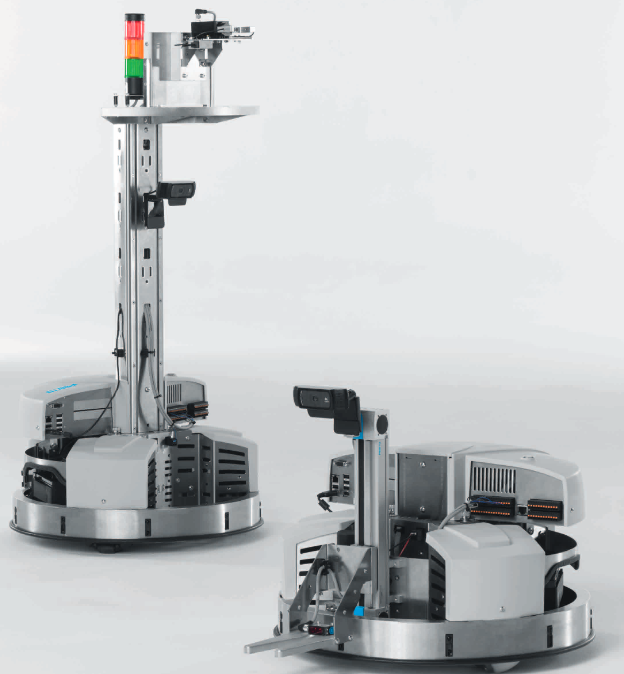
\includegraphics[scale=0.3]{Figures/RobotinoFESTO_base+torre.png}                 
                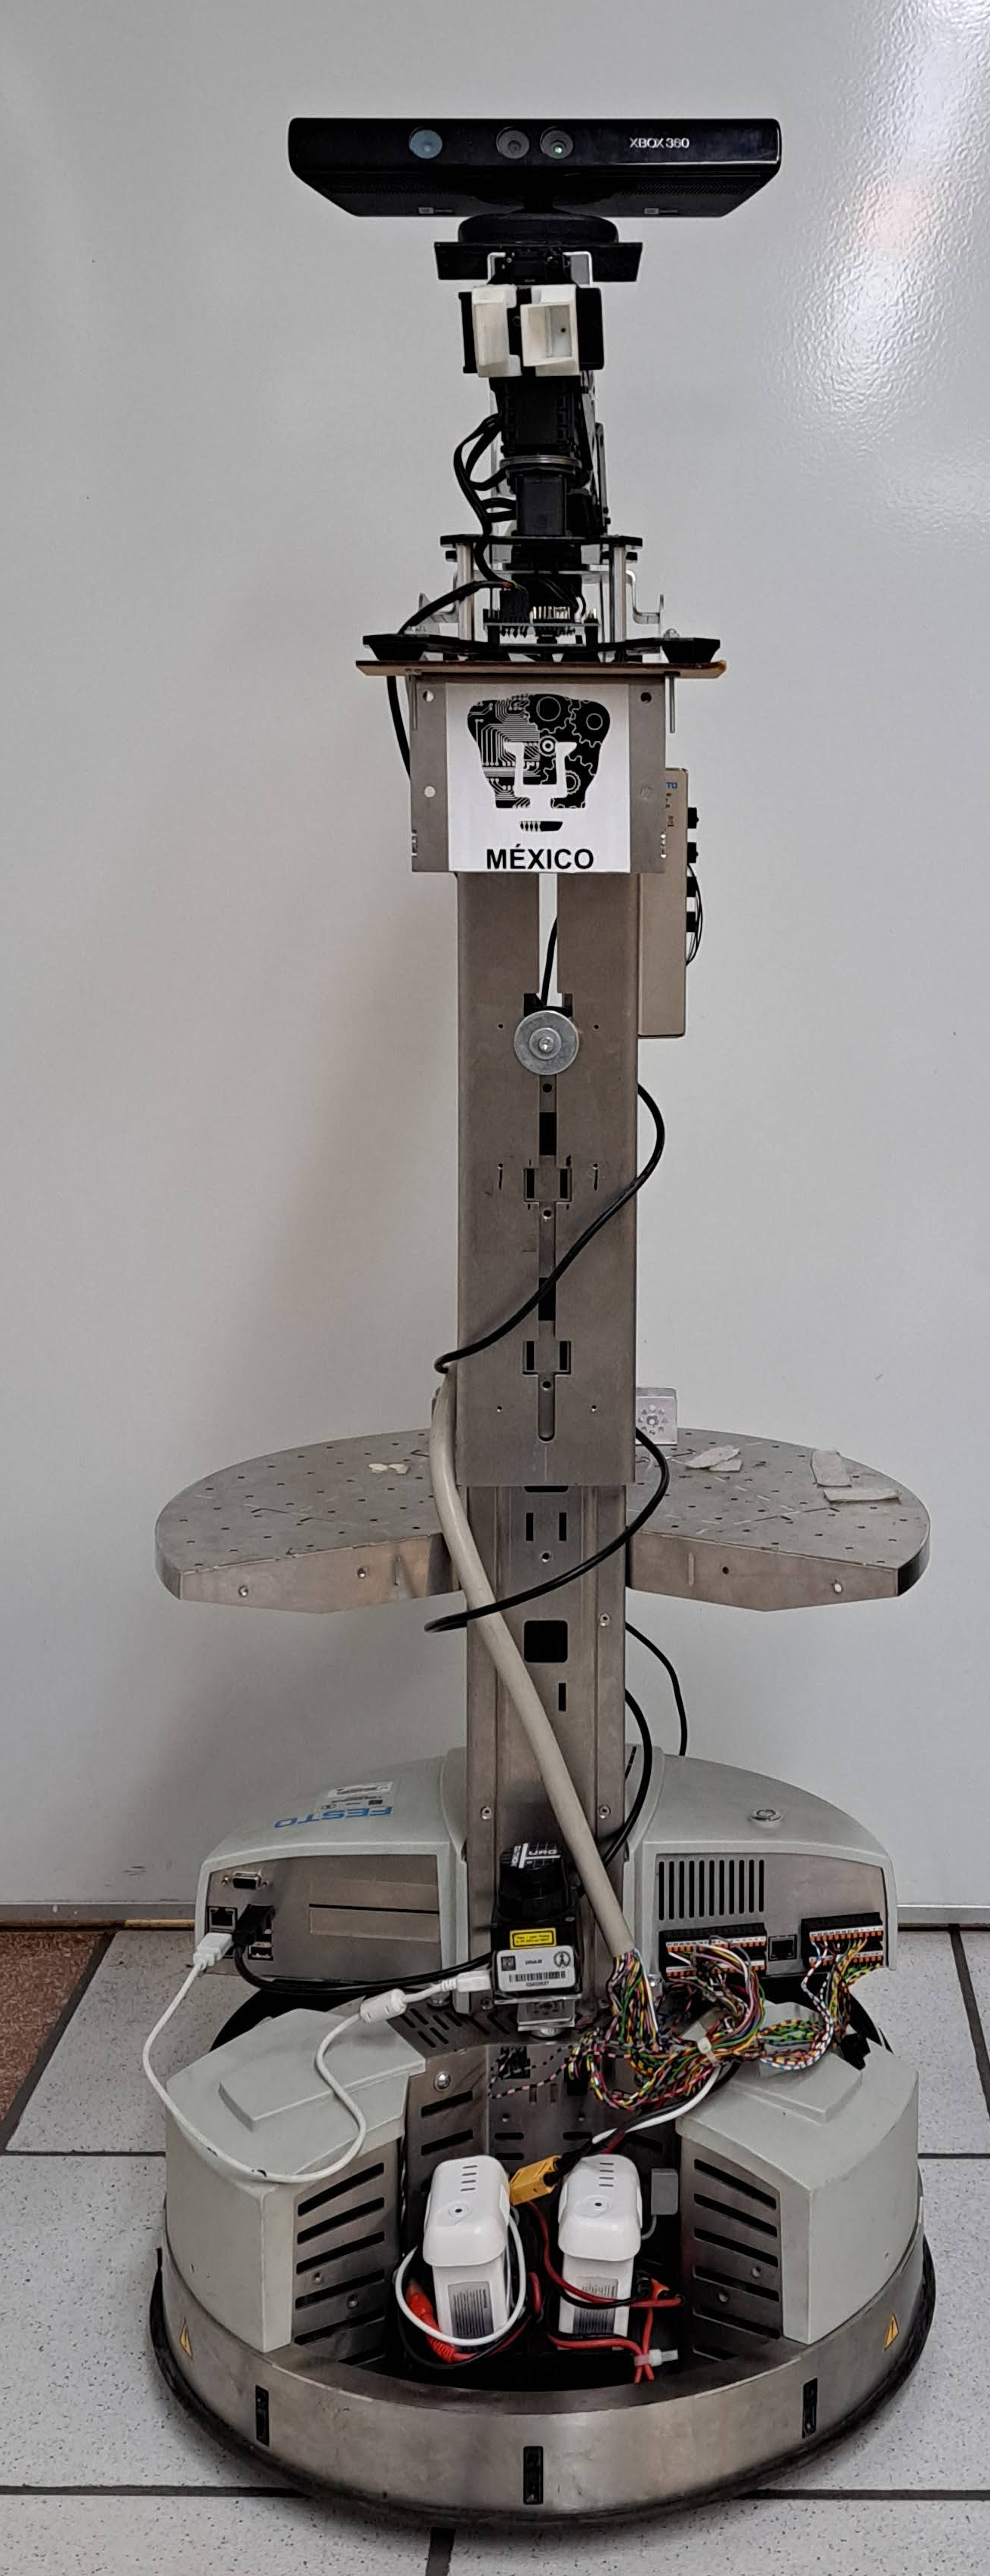
\includegraphics[scale=0.05]{Figures/Robotino_New_New.png}
                    \caption{Robotino 3 \cite{festo-didactic-robotino-2013}}
                    \label{fig:Robotino}
            \end{figure}
                            
            \subsubsection{Camara RGBD - Kinect}

            El autor Vangos Pterneas, ganador del reconocimiento \textit{Microsoft Most Valuable Professional (2014-2019)}, \cite{pterneas_mastering_2022} realiza una descripción del dispositivo Azure Kinect (Microsoft, 2019), así como un análisis de su impacto en la tecnología actual y las herramientas de hardware que le permiten a este aparato ser tan ampliamente utilizado, dando también una descripción de sus antecesores, los dispositivos \textit{HoloLens}, \textit{Kinect versión 2} y \textit{Kinect versión 1}.
            El autor narra que en 2009 Microsoft lanzó al mercado el dispositivo llamado \textit{Project Natal}, cambiando el nombre a \textbf{Kinect} en 2010 y distribuyéndolo como un accesorio para la consola de videojuegos \textit{XBOX 360}. Este dispositivo es capaz de reconocer las partes del cuerpo de las personas y entender sus voces en tiempo real, creando una interfaz interactiva que permitía a los usuarios utilizar la consola sin necesitar un control físico. Para el proyecto que este documento describe, se utilizó la versión 1 del Kinect, mostrado en la figura \ref{fig:Kinect_Parts}, donde también se observan los componentes del dispositivo.

            \begin{figure}[ht]
                \centering
                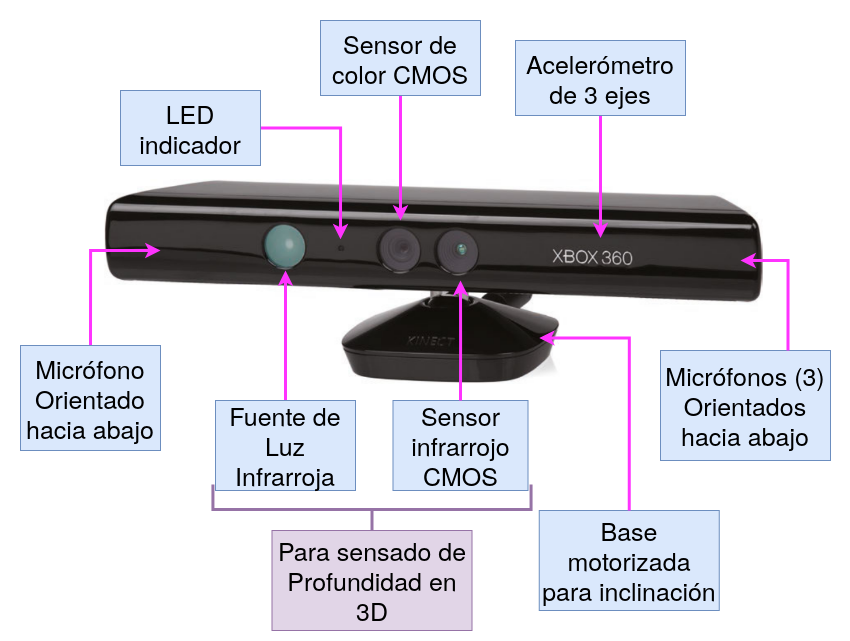
\includegraphics[scale=0.3]{Figures/Kinect_parts.png}
                \caption{Kinect versión 1 - Componentes}
                \label{fig:Kinect_Parts}
            \end{figure}

            \begin{itemize}
                \item Sensor de Profundidad \\
                En \cite{kramer_hacking_2012} Kramer et.al. especifican que el dispositivo Kinect utiliza una cámara MT9M001 (ver figura \ref{Kinect_Sensors}) de la compañía Micron \cite{micron_12-inch_2004}, siendo esta una cámara monocromática con un arreglo de $1280\times1024$ píxeles, aunque estas dimensiones son modificadas antes de la reducción de resolución que se realiza posteriormente.
                Por su parte Davison, en \cite{davison_kinect_2012} describe sus especificaciones, explicando que el sensor de profundidad del Kinect consiste en una fuente de luz infrarroja que proyecta un patrón de puntos, los cuales son leídos después por un sensor infrarrojo CMOS, que detecta los segmentos reflejados del patrón de puntos, además de convertir sus intensidades a distancias. En  \cite{kramer_hacking_2012} se añade que el sensor infrarrojo crea un patrón ruidoso de luz infrarroja estructurada de 830 [nm]. El rango de profundidad del sensor tiene un alcance de 50 [cm] a 3 [m], con una resolución de alrededor de 1 [cm] sobre el eje Z, mientras que la resolución espacial (sobre los ejes X e Y) se encuentra en el orden de los milímetros. Mientras que \cite{davison_kinect_2012} también se explica que cada cuadro generado por el sensor de profundidad cuenta con una resolución de (640 $\times$ 480 píxeles), siendo capaz de mostrar 11 valores de profundidad de 11 bits, dando como resultado 2048 niveles de sensibilidad.

                \begin{figure}[ht]
                    \centering
                    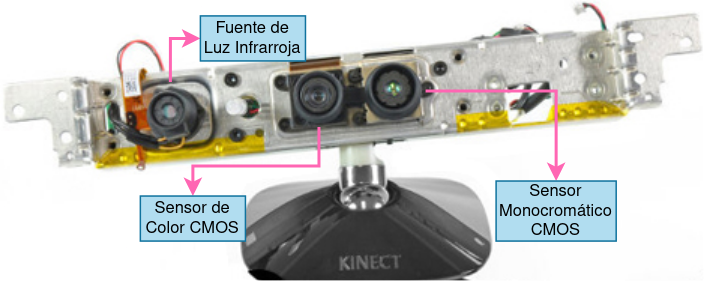
\includegraphics[scale=0.35]{Figures/Kinect_open.png}
                    \caption{Proyector Infrarrojo y Sensores CMOS \cite{eetimes_inside_2010}}
                    \label{fig:Kinect_Sensors}
                \end{figure}


            \begin{table}
                \centering
                \begin{tabular}{|c|c|}
                \hline
                \multicolumn{2}{|c|}{\textbf{Nube de Puntos}} \\
                \hline
                    Rango de Profundidad & 0.8 [m] a 3.5 [m]\\
                \hline
                    Resolución de la nube de puntos & 640 $\times$ 480 píxeles\\
                \hline
                    Niveles de profundidad & 2048\\
                \hline
                    Frecuencia de salida - Nube de puntos & 30 [Hz] \\
                \hline
                    Campo de visión horizontal & 58 \textdegree \\
                \hline
                    Campo de visión vertical & 45 \textdegree \\
                \hline
                    Campo de visión diagonal & 70 \textdegree \\
                \hline
                    Campo de visión horizontal & 58 \textdegree \\
                \hline
                \multicolumn{2}{|c|}{\textbf{Cámara RGB}} \\
                \hline
                \multicolumn{2}{|c|}{Modo \textit{Low Resolution}} \\
                \hline
                    Frecuencia de publicación & 30 [Hz] \\
                \hline
                    Resolución de Imagen & $640\times512$ \\
                \hline
                \multicolumn{2}{|c|}{Modo \textit{High Resolution}} \\
                \hline
                    Frecuencia de publicación & 15 [Hz] \\
                \hline
                    Resolución de Imagen & $1280\times1024$ \\
                \hline
                \multicolumn{2}{|c|}{\textbf{Micrófonos (4)}} \\
                \hline
                    Resolución  & 16 bits\\
                \hline
                    Frecuencia de muestreo & 16 [KHz]\\
                \hline
                
                \hline
                \end{tabular}
                \caption{Especificaciones - Kinect V1}
                \label{tab:Kinect_especs}
            \end{table}

            \item Cámara de video RGB \\
            De acuerdo con Kramer et.al (2012) \cite{kramer_hacking_2012} el dispositivo Kinect contiene una cámara RGB que, de acuerdo con Bob Widenhofer en \cite{eetimes_inside_2010}, utiliza un sensor MT9M112 (ver figura \ref{Kinect_Sensors}). Kramer y su equipo especifican que la cámara opera a 30 [Hz] enviando imágenes de $640\times512$ píxeles. Sin embargo, es posible utilizar una configuración \textit{High Resolution}, que opera a una frecuencia de 15 cuadros por segundo, con imágenes de $1280\times1024$ píxeles. Los autore mencionan también que la cámara cuenta con balance de blancos automático, prevención de parpadeo, saturación de color, referencia de negros y correción de defectos. Los autores también resaltan que ninguno de los dos dispositivos anteriores es de verdadesa utilizad a menos de que se encuentren correctamente calibrados. 
            \end{itemize}
            
            \subsubsection{Manipulador PhantomX Pincher AX-12}
            El manipulador utilizado para este proyecto es el brazo robótico \textbf{PhantomX Pincher AX-12} distribuido por la empresa \textit{Trossen Robotics (Interbotix)}, conocida por poner a disposición del público hardware y software \textit{open source} utilizado en robótica para uso educativo, profesional o de entretenimiento. Los dispositivos de Interbotix se encuentran construidos con servomotores DYNAMIXEL X-Series, y se pueden obtener en configuraciones de 4, 5 o 6 grados de libertad, y es posible controlarlos mediante el Middleware ROS \cite{Interbotix_interbotix}. 
            
            De acuerdo con la información del fabricante \cite{Interbotix_widowx_PincherArm}, este dispositivo es un brazo robótico de 4 grados de libertad, diseñado para se compatible con la plataforma robótica \textit{TurtleBot} de ROS y cuenta con los elementos necesarios para usarlo ya sea como un elemento independiente o bien, como en este caso, integrarlo dentro de otra plataforma robótica. En la figura \ref{fig:Phantom_Pincher} se muestra un ejemplo del manipulador y, a continuación, una descripción del mismo:
            \phantom{saltodelineaforzado >:D}\\
            
            \textbf{Características}
            \begin{itemize}
                \item Actuadores Dynamixel AX-12A 
                \item Base sólida con rodamiento de agujas. Construcción resistente en Delrin/acrílico.
                \item Controlador robótico Arbotix para procesamiento integrado
                \item Pinza paralela personalizable
                \item Soportes de montaje para cámaras y sensores
            \end{itemize}
            
            \phantom{saltodelineaforzado >:D}\\
            
            \textbf{Especificaciones}
            \begin{itemize}
                \item Peso: 550 [g]
                \item Alcance Vertical: 35 [cm]
                \item Alcance Horizontal: 31 [cm]
                \item Fuerza:
                \begin{itemize}
                    \item 25[cm]/ 40[g]
                    \item 20[cm]/ 70[g]
                    \item 15[cm]/ 100[g]
                \end{itemize}
                \item Fuerza de agarre de la pinza: 500 [g]
                \item Fuerza de levantamiento de la muñeca: 250[g]
            \end{itemize}

            \begin{figure}[H]
                \centering
                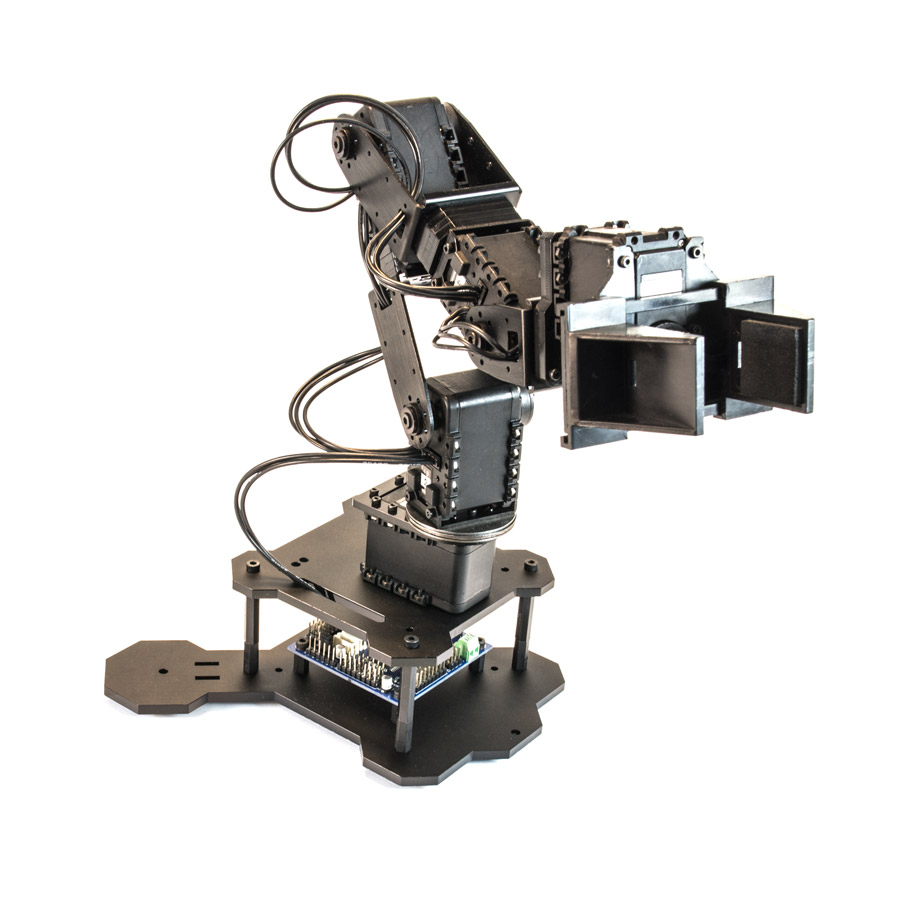
\includegraphics[scale=0.2]{Figures/Phantom_Pincher.jpg}
                    \caption{PhantomX Pincher AX-12}
                    \label{fig:Phantom_Pincher}
            \end{figure}
Para lograr la integración de todos los elementos anteriormente mencionados, el desarrollo se realizó utilizando una combinación de los lenguajes C++ y Python. 
\subsection{}
La evaluación del resultado de esta implementación se dio parcialmente durante la competencia RoboCup 2023, donde se cuenta con las estaciones de trabajo y el set de piezas completas. durante esta evaluación bajo condiciones reales fue posible observar debilidades en la implementación que fueron cubiertas posteriormente.
